\section{Определения}

\subsection{Множество, основные теоретико-множественные операции, упорядоченная пара, декартово произведение.}
\
\begin{enumerate}
    \item \textit{Множеством} называется произвольный набор (совокупность, класс, семейство) каких-либо объектов. Объекты, входящие во множество, называются его \textit{элементами}. Если объект $x$ является элементом множества $A$, то говорят, что $x$ принадлежит $A$, и пишут $x \in A$.
    \item Множество $A$ является \textit{подмножеством} множества $B$, если любой элемент множества $A$ также принадлежит множеству $B$. Обозначение: $A \subset B$.
    \item Множества $A$ и $B$ \textit{равны}, если одновременно $A \subset B$ и $B \subset A$. Обозначение: $A = B$.
    \item  Для задания \textit{упорядоченной пары} нужно задать неупорядоченную и первый элемент в ней. Например, по упрощённому определению Куратовского: $(a, b) = \{a, \{a, b\}\}$.
    \item \textit{Кортежем} длины 0 называется пустое множество. Если уже задан $T = (a_{1}, \ldots, a_{n})$ -- кортеж длины $n$, то $(a, a_{1}, \ldots, a_{n}) = \{a, \{a, T\}\}$ есть кортеж длины $n + 1$. Так можно получить ещё одно определение упорядоченной пары: $(a, b) = \{a, \{a, \{b, \{b, \emptyset\}\}\}\}$.
    \item \textit{Декартовым произведением} множеств $A$ и $B$ называется множество упорядоченных пар $A \times B = \{(a, b) \ | \ a \in A, b \in B\}$. \textit{Декартовой степенью} $A^n$ множества $A$ называется множество кортежей длины $n$ из элементов $A$.
\end{enumerate}

\begin{itemize}
    \item \textit{Объединением} $A$ и $B$ называется множество $A \cup B = \{x \ | \ x \in A \text{ или } x \in B\}$.
    \item \textit{Пересечением} $A$ и $B$ называется множество $A \cap B = \{x \ | \ x \in A \text{ и } x \in B\}$.
    \item \textit{Разностью} $A$ и $B$ называется множество $A \backslash B = \{x \ | \ x \in A \text{ и } x \not\in B\}$.
    \item \textit{Симметрической разностью} $A$ и $B$ называется множество $A \triangle B = (A \backslash B) \cup (B \backslash A)$.
    \item \textit{Дополнением} множества $A$ называется множество $A = \{x \ | \ x \not\in A\}$.
\end{itemize}

\subsection{Отображения и соответствия. Образ и прообраз. Инъекции, сюръекции, биекции. Композиция отображений. Возведение множества в степень множества.}

\begin{enumerate}
    \item \textit{Соответствием} между множествами $A$ и $B$ называют произвольное подмножество декартова произведения $F \subset A \times B$.
    \item \textit{Отображением} из множества $A$ в множество $B$ называется однозначное соответствие между $A$ и $B$, т. е. такое соответствие, что для любого $a \in A$ найдётся ровно одно $b \in B$, соответствующее $a$.
    \item Соответствие $F$ называется \textit{инъективным}, если для любых $a_1 \neq a_2$ множества $F(a_1)$ и $F(a_2)$ не пересекаются. Инъективное отображение называется \textit{инъекцией}.
    \item Соответствие $F$ называется \textit{сюръективным}, если любой элемент $B$ соответствует хотя бы одному элементу $A$, т. е. любой $b \in B$ лежит в $F(a)$ для некоторого $a \in A$. Сюръективное отображение называется \textit{сюръекцией}.
    \item \textit{Биекцией} называется отображение, являющееся одновременно инъекцией и сюръекцией.
    \item Пусть $F: A \rightarrow B$ -- соответствие, а $S \subset A$. \textit{Образ} $S$ -- это множество $F(S) = \bigcup_{s \in S} F(s) \subset B$.
    \item Пусть $F: A \rightarrow B$ -- соответствие, а $T \subset B$. \textit{Проообраз} $T$ -- это множество $F^{-1}(T) = \{a \ | \ F(a) \cap T \neq \emptyset\} \subset A$.
    \item Пусть $F: A \to B$ и $G: B \to C$ -- соответствия. Тогда их \textit{композицией} $G \circ F$ называется соответствие $H: A \to C$, определенное правилом: $c \in H(a)$ тогда и только тогда, когда найдется $b$, такое что одновременно $c \in G(b)$ и $b \in F(a)$.
    \item Пусть $A$ и $B$ -- два множества. Тогда множеством $B^A$ называется множество всех отображений из $A$ в $B$.
\end{enumerate}

\subsection{Равномощность. Счётные и континуальные множества.}

\begin{enumerate}
    \item Множества $A$ и $B$ назваются \textit{равномощными}, если существует биекция $A \to B$. Обозначение: $A \cong B$.
    \item Множество $A$ называется \textit{счетным}, если оно равномощно множеству $\N$.
    \item Множество $A$ называется \textit{континуальным}, если оно равномощно множеству $\R$.
\end{enumerate}

\subsection{Бинарные отношения. Рефлексивность, транзитивность, (анти)симметричность и т. д. Отношения эквивалентности и отношения порядка.}

\textbf{Определение:} \textit{Бинарным отношением} на множестве $A$ называется любое подмножество $R \subset A \times A$.

\begin{center}
    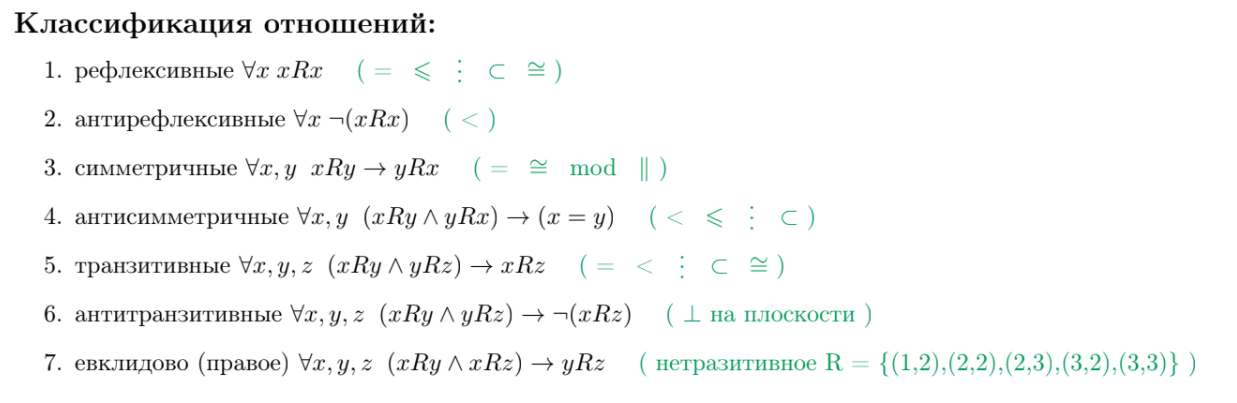
\includegraphics[width = 0.92\textwidth]{images/2 (определения)_m22.PNG}

    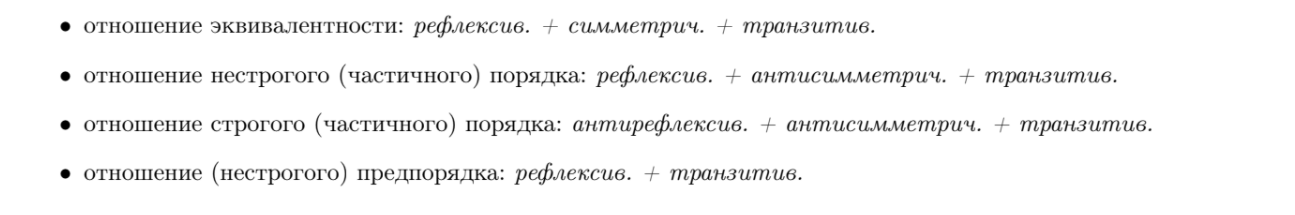
\includegraphics[width = 0.93\textwidth]{images/2 (определения)_m23.PNG}
\end{center}

\subsection{Упорядоченное множество, линейно упорядоченное множество, фундированное множество, вполне упорядоченное множество.}

\textbf{Определение:} \textit{Упорядоченым множеством} называется пара $(A, \leq_A)$ -- множество и отношение порядка на нем.

\textbf{Определение:} Частично упорядоченное множество называется \textit{линейно упорядоченным}, если любые два элемента в нем сравнимы.

\textbf{Определение:} Частично упорядоченное называется \textit{фундированным}, если в любом его непустом подмножестве есть минимальный элемент.

\textbf{Пример}
\begin{itemize}
    \item [$\checkmark$] $\langle\mathbb{N}, \leq\rangle$, $\langle\mathbb{N} + \mathbb{N}, \leq\rangle$, $\langle\mathbb{N},|\rangle$ с заданным тривиально порядком -- фундированные.
    \item [$\times$] $\mathbb{Z}$, $[0,1]$ -- не фундированные.
\end{itemize}

\textbf{Определение:} Фундированное линейно упорядоченное множество называется \textit{вполне упорядоченными}, а соответствующий порядок -- полным.

\textbf{Пример}
\begin{itemize}
    \item [$\times$ ] Множество всех конечных слов из букв латинского алфавита.
    \item [$\times$ ] [0,1], $\langle \mathbb{N},|\rangle$.
    \item [$\checkmark$ ] $\mathbb{N}$.
\end{itemize}

\subsection{Цепи в упорядоченных множествах. Верхние и нижние грани, максимальные и минимальные, наибольшие и наименьшие элементы.}

\textbf{Определение:} Подмножество частично упорядоченного множества называется \textit{цепью}, если любые два его элемента сравнимы.

\textbf{Определение:} Элемент $a \in M$ называется \textit{минимальным}, если $b \leq a$ только при $b = a$. Элемент $a \in M$ называется \textit{наименьшим}, если $\forall b\in M: a \leq b$.
Аналогично вводятся понятия \textit{максимального} и \textit{наибольшего} элементов.

\textbf{Определение:} \textit{Верхней гранью} множества $A$ называется такой элемент $M$, что $\forall x \in A: \ x\leq M$.

\textbf{Определение:} \textit{Нижней гранью} множества $A$ называется такой элемент $m$, что $\forall x \in A: \ x\geq m$.

\subsection{Гомоморфизмы и изоморфизмы упорядоченных множеств.}

\textbf{Определение:} \textit{Гомоморфизмом упорядоченных множеств} называется функция $f:A\rightarrow B$, такая что
\begin{center}
    $x \leq_A y \lra f(x) \leq_B f(y)$.
\end{center}

\textbf{Определение:} \textit{Изоморфизмомом  упорядоченных множеств} называется  функция $f:A\rightarrow B$, являющаяся гомоморфизмом и биекцией.

\subsection{Сложение и умножение упорядоченных множеств.}

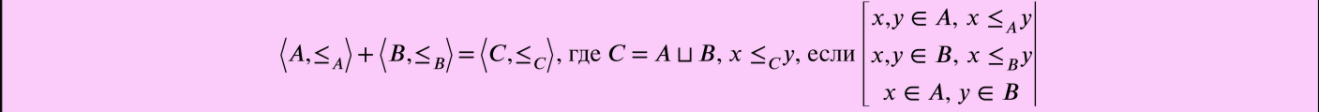
\includegraphics[width = 0.94\textwidth]{images/2 (определения)_m24.PNG}


\includegraphics[width = 0.94\textwidth]{images/2 (определения)_m25.PNG}

\subsection{Начальные отрезки вполне упорядоченных множеств.}
\textbf{Определение:} Пусть $S$ -- ВУМ. Подмножество $A \subset S$ называется \textit{начальным отрезком}, если $\forall x \forall y \left((x \leq y \land y \in A) \to x \in A \right)$.

\textbf{Примеры}
\begin{itemize}
    \item [$\checkmark$] $[0,a] = \{x \ | \ x\leq a\}$.
    \item [$\checkmark$] $[0,a) = \{x \ | \ x<a\}$.
    \item [$\checkmark$] Всё $S$.
\end{itemize}

\subsection{Предельные элементы вполне упорядоченных множеств.}

\textbf{Определение:} В любом ВУМ у любого элемента $a$, кроме максимального, есть единственный \textit{непосредственно следующий} за ним (элемент $a + 1$), т.е. такой $c > a$, что не существует такого $b$, что $a < b < c$.

\textbf{Определение:} \textit{Предельным элементом} ВУМ называется элемент, не являющийся непосредственно следующим ни для какого другого элемента.

\subsection{Порядковые типы $\omega, \omega^k, \omega^{\omega}, \epsilon_0$.}

\textbf{Определение:} Неформально \textit{ординалом} (порядковым числом или порядковым типом) называется
класс эквивалентности вполне упорядоченных множеств по отношению изоморфности. Формально ординалом называется транзитивное множество, каждый элемент которого также транзитивен.

Будем обозначать $0$ -- порядковый тип пустого множества, $1$ -- порядковый тип множества из одного элемента, $k$ -- порядковый тип линейного порядка на $k$-элементном множестве (такие ординалы называются конечными), $\omega$ -- порядковый тип множества натуральных чисел $\N$ со стандартным порядком.

Рассмотрим порядковый тип $\omega$. Следующим за ним будет $\omega + 1$, потом $\omega + 2, \ldots, \omega + \omega = \omega \cdot 2, \omega \cdot 2 + 1, \ldots, \omega \cdot 3, \ldots, \omega \cdot \omega = \omega^2$. Далее идут $\omega^2 + 1, \ldots, \omega^2 + \omega, \ldots, \omega^{2}\cdot 2, \ldots, \omega^3, \ldots, \omega^\omega, \ldots, \omega^{\omega + 1}, \ldots, \omega^{\omega^{\omega}}, \ldots, \epsilon_{0} = \omega^{\omega^{\omega^{\ldots}}}$($\omega$ раз).

$\epsilon_0$ -- минимальный ординал, такой что $\epsilon_0 = \omega^{\epsilon_0}$.

\subsection{Аксиома выбора.}

Пусть задано некоторое множество $A$. Тогда существует функция $\phi: 2^A \setminus \{A\} \rightarrow A$ такая, что $\forall S \subset A:\ \phi(S) \in S$.

\subsection{Базис Гамеля.}

Базис Гамеля в $\mathbb R$ над $\Q$ это такой набор действительных чисел, что любое другое действительное число представляется как конечная линейная комбинация элементов базиса с рациональными коэффициентами, при этом никакая нетривиальная конечная линейная комбинация элементов базиса с рациональными коэффициентами не равна $0$.